\documentclass{beamer}
\title{Welcome to Beamer}
\author{You}
\institute{Where You're From}
\date{Date of Presentation}
\begin{document}
\begin{frame}

\tableofcontents[currentsection]
\end{frame}

\begin{frame}

\titlepage
% beamer's \maketitle
\end{frame}
\begin{frame}
\frametitle{Presentations with beamer: Frames}
\begin{itemize}
\item Use \texttt{frametitle} to give the frame a title.
\item Then add content to the frame.
\item The source for this frame looks like ...
\end{itemize}
\end{frame}

\begin{frame}

\begin{columns}
\begin{column}{0.4\textwidth}
\begin{itemize}
\item Use the columns ...
\item The argument ...
\item See also the ...
\end{itemize}
\end{column}
\begin{column}{0.6\textwidth}
% second column
\end{column}
\end{columns}
\end{frame}

\begin{frame}
I should \emph{emphasise} that
this is an \alert{important} point.

Text in \textbf{bold face}.
Text in \textit{italics}.

It \textcolor{red}{stops}
and \textcolor{green}{starts}.

\end{frame}

\begin{frame}
\begin{figure}
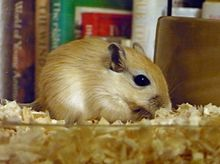
\includegraphics[
width=0.5\textwidth]{gerbil}
\end{figure}
\end{frame}

\begin{frame}
\begin{tabular}{lrr}
Item   & Qty & Unit \$ \\
Widget & 1   & 199.99  \\
Gadget & 2   & 399.99  \\
Cable  & 3   & 19.99   \\
\end{tabular}
\end{frame}

\begin{frame}
\begin{block}{Interesting Fact}
This is important.
\end{block}
\begin{alertblock}{Cautionary Tale}
This is really important!
\end{alertblock}
\end{frame}

\end{document}